\textbf{Problem 6}

\textbf{NOTE: }All referenced figures and tables can be found on the next 4 pages.

a) Run ``python3 q6.py'' to run one simulation of the program. You must install the numpy and matplotlib libraries, which can be done through the following commands: ``pip3 install numpy'' and ``pip3 install matplotlib''.

b) Results can be seen in Tables \ref{mh-table-05}, \ref{mh-table-5}, as well as Figures \ref{mh-figure-05}, \ref{mh-figure-5}. While both values of $\sigma$ produce the correct estimated means (-5 and 5), their acceptance rates are vastly different. With $\sigma = 0.5$, we get an acceptance rate of 0.1303. Meanwhile, with $\sigma = 5$, we get acceptance rate 0.0025. This makes sense since with a smaller value of $\sigma$, the random walk of the MH algorithm (which is produced by the proposal distribution) leads us to making smaller steps. Meanwhile, when the value of $\sigma$ is larger, those steps are going to be larger at each iteration, which means there is a higher chance of making a step in the wrong direction, thus leading to a larger rejection rate by the algorithm. Basically, smaller $\sigma$ means smaller, more precise, and subsequently more confident steps.

c) Results can be seen in Table \ref{gibbs-table} and Figure \ref{gibbs-figure}. The estimated means are roughly where they should be (-5 and 5).

\pagebreak \begin{table}[h]
	\centering
	\begin{tabular}{|c|l|l|l|}
		\hline
		\textbf{Simulation \#} & $\mathbf{\mu_1}$     & $\mathbf{\mu_2}$    & \textbf{Acceptance Rate} \\ \hline
		1 & -5.0212 & 5.0119 & 0.1225               \\ \hline
		2 & -5.1669 & 5.1004 & 0.1296               \\ \hline
		3 & -4.8128 & 4.9267 & 0.1310               \\ \hline
		4 & -5.0322 & 5.0308 & 0.1335               \\ \hline
		5 & -5.2505 & 4.8600 & 0.1309               \\ \hline
		6 & -5.0585 & 4.9253 & 0.1340               \\ \hline
		\textbf{Average} & -5.0570 & 4.9759 & 0.1303               \\ \hline
	\end{tabular}
	\caption{Metropolis-Hastings with $\sigma = 0.5$}
	\label{mh-table-05}
\end{table}

\begin{table}[h]
	\centering
	\begin{tabular}{|l|l|l|l|}
		\hline
		\textbf{Simulation \#} & $\mathbf{\mu_1}$     & $\mathbf{\mu_2}$    & \textbf{Acceptance Rate} \\ \hline
		1             & -4.9132 & 4.8871 & 0.0025          \\ \hline
		2             & -4.9984 & 4.9574 & 0.0019          \\ \hline
		3             & -5.3520 & 4.8601 & 0.0030          \\ \hline
		4             & -5.1066 & 4.8501 & 0.0029          \\ \hline
		5             & -5.2658 & 4.8183 & 0.0023          \\ \hline
		6             & -5.1072 & 5.0082 & 0.0023          \\ \hline
		\textbf{Average}       & -5.1239 & 4.8969 & 0.0025          \\ \hline
	\end{tabular}
	\caption{Metropolis-Hastings with $\sigma = 5$}
	\label{mh-table-5}
\end{table}

\begin{table}[h]
	\centering
	\begin{tabular}{|l|l|l|}
		\hline
		\textbf{Simulation \#} & $\mathbf{\mu_1}$     & $\mathbf{\mu_2}$    \\ \hline
		1 & -5.0954 & 5.0613 \\ \hline
		2 & -4.7688 & 4.8494 \\ \hline
		3 & -4.9848 & 4.9554 \\ \hline
		4 & -5.2155 & 4.8305 \\ \hline
		5 & -5.0172 & 4.8701 \\ \hline
		6 & -4.9543 & 4.9489 \\ \hline
		\textbf{Average} & -5.0060   & 4.9193 \\ \hline
	\end{tabular}
	\caption{Gibbs Sampling}
	\label{gibbs-table}
\end{table}

\begin{figure}
	\centering
	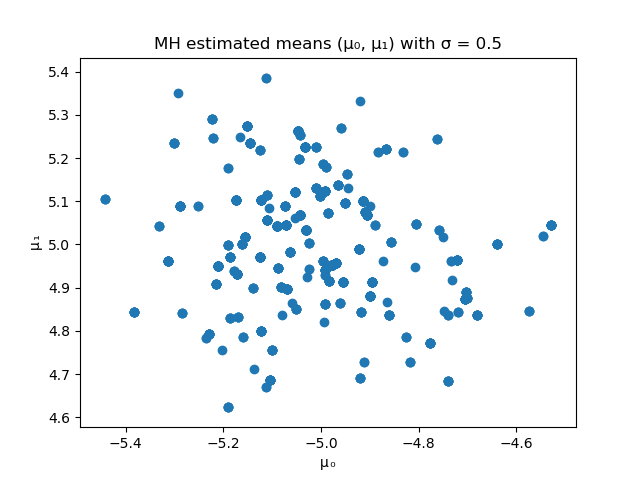
\includegraphics[scale=0.5]{mh-estimated-means-with-sigma-05-1.png}
	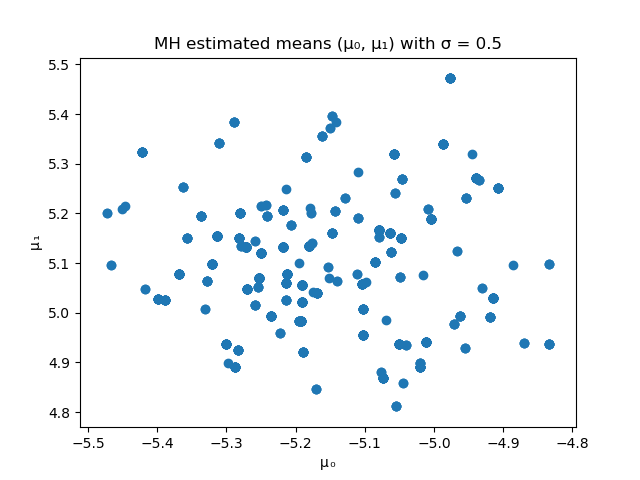
\includegraphics[scale=0.5]{mh-estimated-means-with-sigma-05-2.png}
	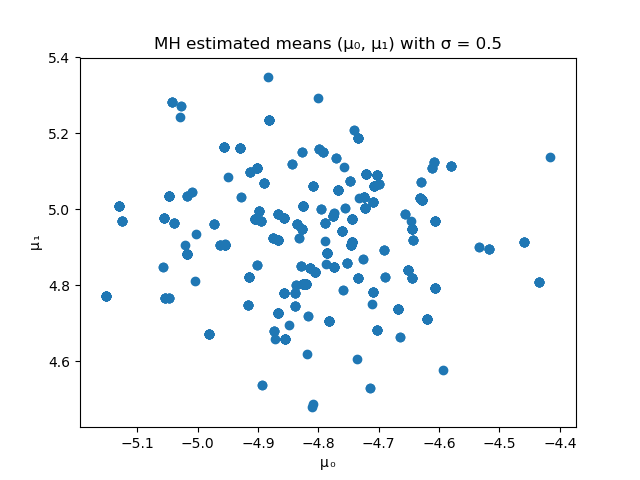
\includegraphics[scale=0.5]{mh-estimated-means-with-sigma-05-3.png}
	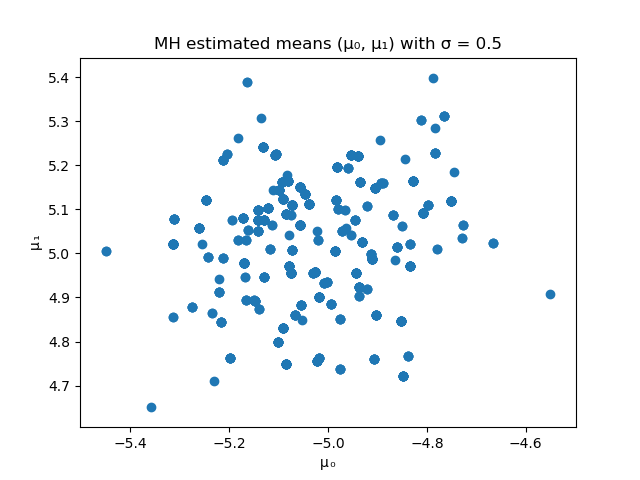
\includegraphics[scale=0.5]{mh-estimated-means-with-sigma-05-4.png}
	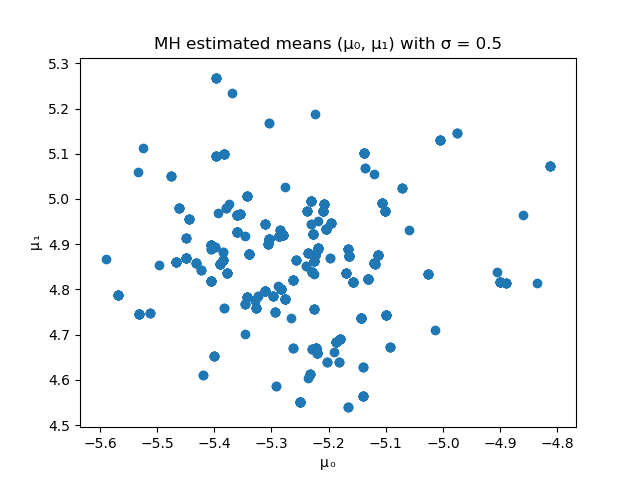
\includegraphics[scale=0.5]{mh-estimated-means-with-sigma-05-5.png}
	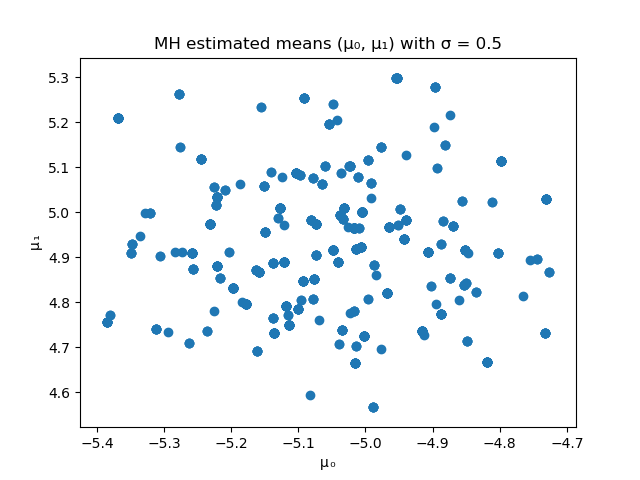
\includegraphics[scale=0.5]{mh-estimated-means-with-sigma-05-6.png}
	\caption{Metropolis-Hastings with $\sigma = 0.5$}
	\label{mh-figure-05}
\end{figure}

\begin{figure}
	\centering
	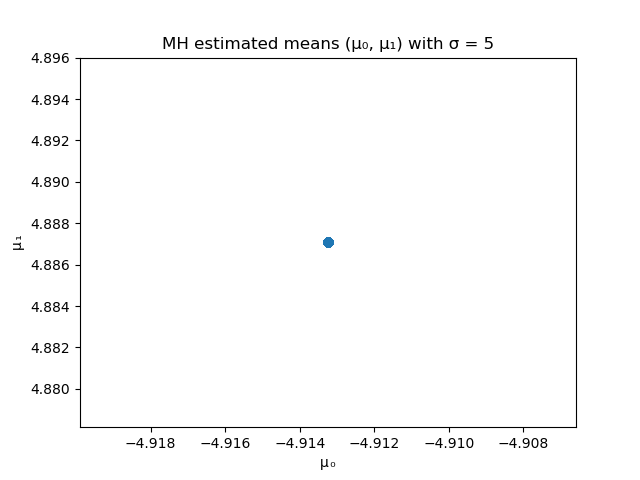
\includegraphics[scale=0.5]{mh-estimated-means-with-sigma-5-1.png}
	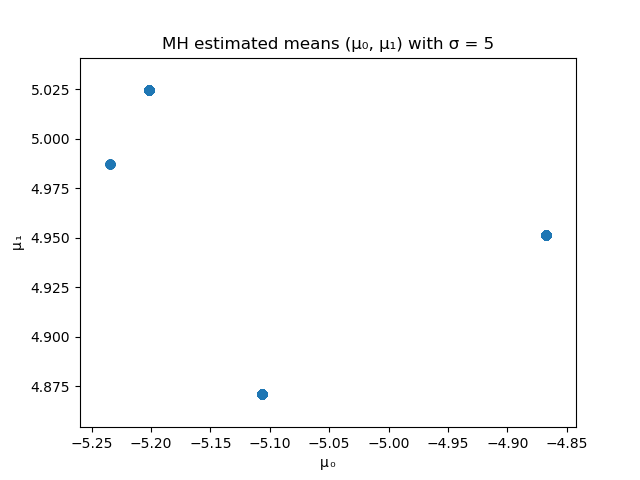
\includegraphics[scale=0.5]{mh-estimated-means-with-sigma-5-2.png}
	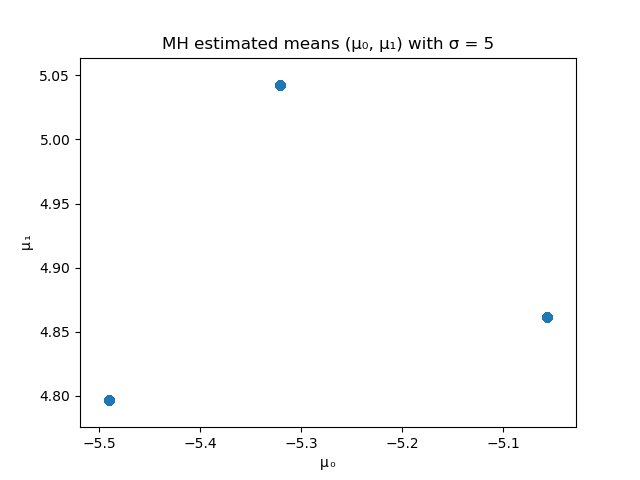
\includegraphics[scale=0.5]{mh-estimated-means-with-sigma-5-3.png}
	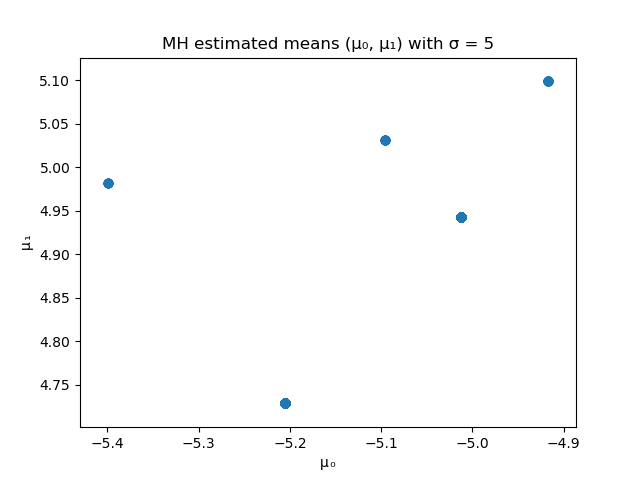
\includegraphics[scale=0.5]{mh-estimated-means-with-sigma-5-4.png}
	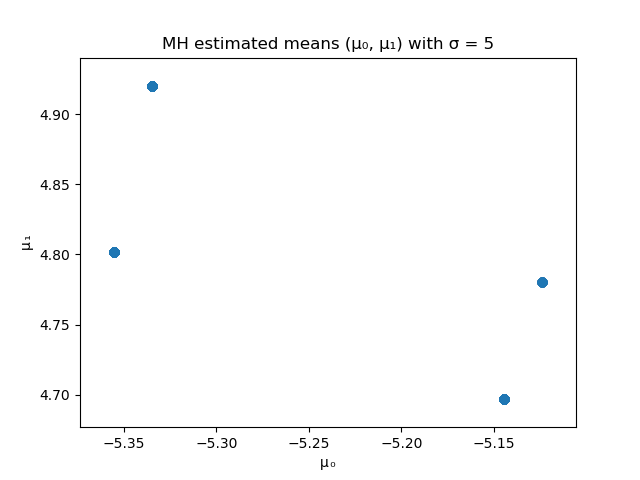
\includegraphics[scale=0.5]{mh-estimated-means-with-sigma-5-5.png}
	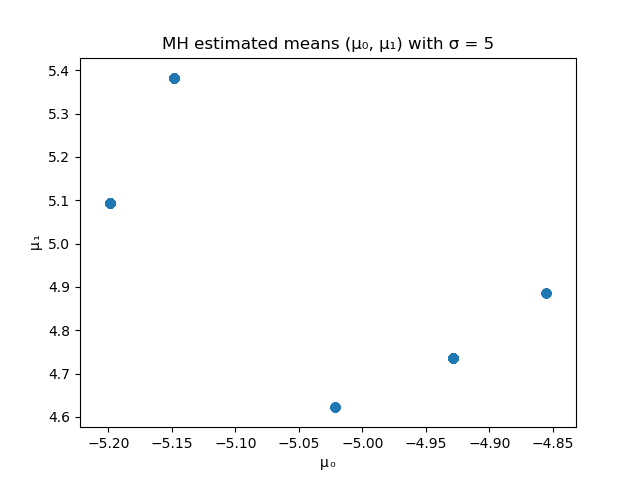
\includegraphics[scale=0.5]{mh-estimated-means-with-sigma-5-6.png}
	\caption{Metropolis-Hastings with $\sigma = 5$}
	\label{mh-figure-5}
\end{figure}

\begin{figure}
	\centering
	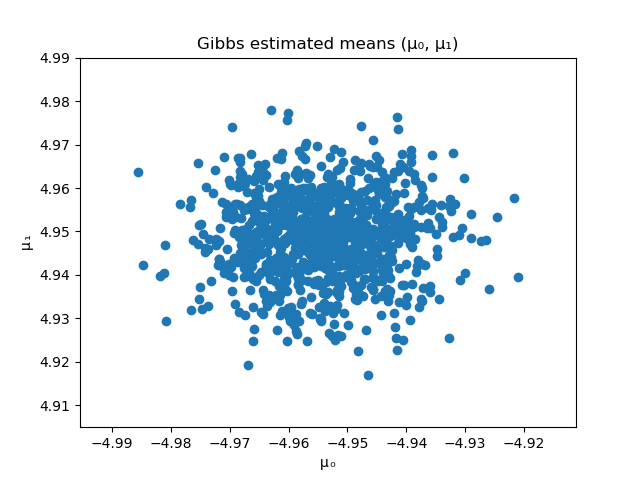
\includegraphics[scale=0.5]{gibbs-estimated-means-1.png}
	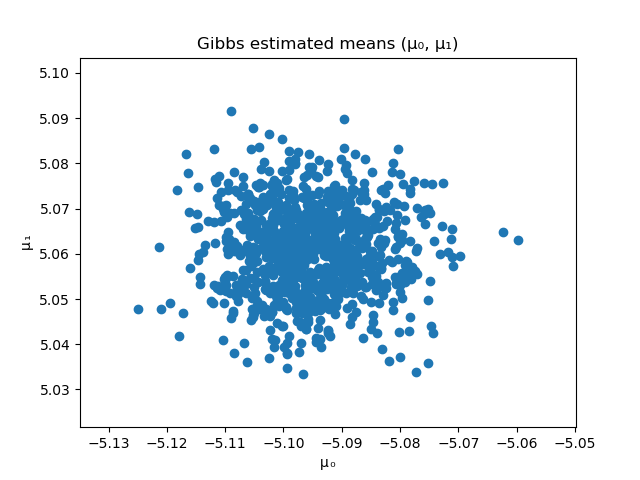
\includegraphics[scale=0.5]{gibbs-estimated-means-2.png}
	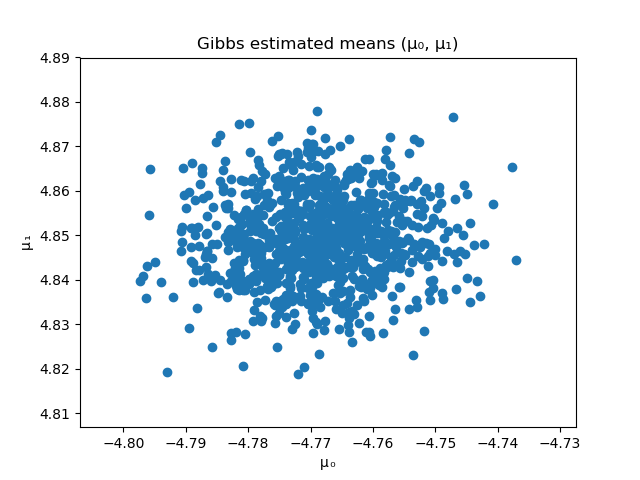
\includegraphics[scale=0.5]{gibbs-estimated-means-3.png}
	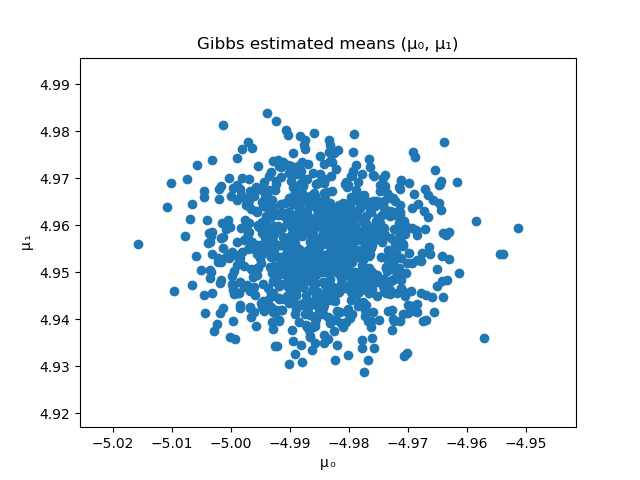
\includegraphics[scale=0.5]{gibbs-estimated-means-4.png}
	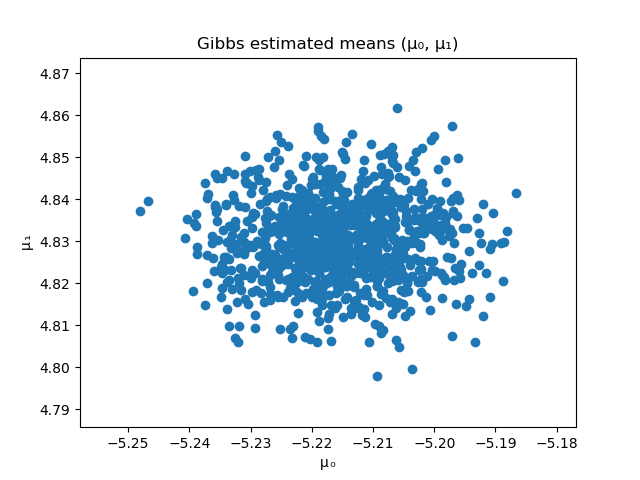
\includegraphics[scale=0.5]{gibbs-estimated-means-5.png}
	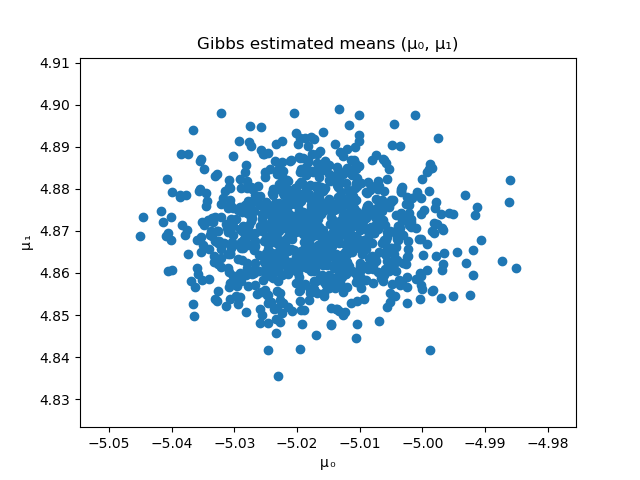
\includegraphics[scale=0.5]{gibbs-estimated-means-6.png}
	\caption{Gibbs Sampling}
	\label{gibbs-figure}
\end{figure}